% !TEX spellcheck = en_US

% !TEX root = elastophi-report.tex


\section{Results}
\label{sec:results}

In this section we report a series of test cases to illustrate the performance of our code on different geometrical structures.
Figures~\ref{fig:450Fracs}--\ref{fig:3600FracsV3DN3} refer to discrete networks of \emph{fractures} (DFN), where each fracture is represented by a mesh element (a quadrangle);    
Figure~\ref{fig:5364FracsTriangles} refers to a network of large \emph{faults}, which have been triangulated and we consider each mesh triangle as a fracture. Both types of structure are considered in IFPEN applications.

\quad\\
For each geometrical structure we show first the corresponding mesh.
Then, for the test cases of smaller dimension (Figures~\ref{fig:450Fracs} and \ref{fig:1363Fracs}), we visualize, for some couples of $\eta$ and $\varepsilon$, the local compression rate of each block of the HM-ACA matrix by coloring its entries using a color scale from $0$ to $1$. The local compression rate of an admissible block of dimension $n\times m$ with rank $k$ in ACA approximation is $1-k(n+m)/(n\cdot m)$ (the larger the compression rate, the more the matrix is compressed); the local compression rate of the non compressed blocks is set to $0$. Note that a block is not necessarily a connected part of the matrix.

\quad\\
For all the cases, an error-compression graph summarizes the relevant results: for certain couples of values of the parameters $\eta$ and $\varepsilon$, on the vertical axis we report the relative error in Frobenius norm of the corresponding HM-ACA matrix with respect to the dense matrix, and on the horizontal axis the achieved global compression rate. Next to each marker we indicate the value of $\varepsilon$ ($\varepsilon=1, 0.9, 0.5, 0.1, 0.01$) and the legend gives the value of $\eta$ ($\eta=10,1,0.1$). The expression ``0 blocks'' means that the admissible blocks are approximated with zero rank matrices (i.e.~zero matrices, but we just need to store $k=0$) instead of computing their ACA approximation.
The global compression rate of a $3N\times 3N$ matrix $A$ is defined as:
\[
1- \Biggl(\sum_{t \times s \in \mathscr{B}}{\frac{k(\lvert t \rvert + \lvert s \rvert)}{3N\cdot3N} } + 
\sum_{t \times s \in \mathscr{B}^c}{\frac{\lvert t \rvert \lvert s \rvert}{3N\cdot3N} } \Biggr),
\]
where $\mathscr{B}$ is the subset of $\llbr 1,3N\rrbr\times \llbr 1,3N\rrbr$ corresponding to admissible (and then compressed) blocks introduced in Section~\ref{section:partition}.

Moreover, for the geometrical structures (Figures~\ref{fig:1994Fracs}, \ref{fig:3600FracsV1DN1}--\ref{fig:3600FracsV3DN3}, \ref{fig:5364FracsTriangles}) for which the sparse matrices obtained by IFPEN with the heuristic method are available, we report with a red triangular marker (``ref'' in the legend) the corresponding relative error in Frobenius norm and compression rate, given by $1- n_{\bar{0}}/(3N\cdot3N)$, where $n_{\bar{0}}$ is the number of non zero coefficients of the sparse matrix.

\quad\\
Finally, in Figures~\ref{fig:1994Fracs} and \ref{fig:5364FracsTriangles}, we include two time-compression graphs to show the relation between the global compression rate and the time (in seconds) for the construction of the HM-ACA matrix and for the matrix-vector product with a (fixed) random generated vector. Remark that the code has not been fully optimized yet, so the computing times can be further improved.  

\quad\\
We observe that when $\varepsilon$ increases, the relative error and the global compression rate increase as expected: recall that $\varepsilon$ is used in the stopping criterion~\eqref{eq:stopCrit} for the ACA compression of each admissible block and the stopping criterion becomes less restrictive with bigger $\varepsilon$. Note that with $\varepsilon \ge 1$ the ACA loop always stops after computing just $1$ rank. 
Similarly, when $\eta$ increases, the relative error and the global compression rate increase: indeed, $\eta$ appears in the admissibility condition~\eqref{AdmissibilityCondition} and a bigger $\eta$ allows the balls $B_t$ and $B_s$ to be farther while maintaining the admissibility of the corresponding block.
However, note that the relative error is much less sensible to the variation of $\varepsilon$ than to the variation of $\eta$.

\quad\\
In Figures~\ref{fig:1994Fracs}, \ref{fig:3600FracsV1DN1}--\ref{fig:3600FracsV3DN3}, \ref{fig:5364FracsTriangles} one can note that the relative error obtained with the HM-ACA matrix is significantly lower than the one with the IFPEN sparse matrix (note that the vertical axis scale is logarithmic), even when the admissible blocks are approximated simply with zero matrices, while maintaining a comparable compression rate. 

For instance, to give some precise values of the results appearing in the graphs, for the structure in Figure~\ref{fig:1994Fracs} with $1994$ fractures, the relative error with the HM matrix with zero blocks and $\eta=1$ is $0.019$ ($1.9 \%$) with compression rate $0.86$, or with the HM-ACA matrix with $\varepsilon=1$ and $\eta=1$ the relative error is $0.012$ ($1.2 \%$) with compression rate $0.68$, while with the IFPEN sparse matrix the relative error is $0.45$ ($45 \%$) with compression rate $0.99$.  
For the structure of faults in Figure~\ref{fig:5364FracsTriangles} the results are even better, for instance 
the relative error with the HM matrix with zero blocks and $\eta=1$ is $0.0055$ ($0.55 \%$) with compression rate $0.98$, or with the HM-ACA matrix with $\varepsilon=1$ and $\eta=1$ the relative error is $0.0038$ ($0.38 \%$) with compression rate $0.92$, while with the IFPEN sparse matrix the relative error is $0.41$ ($41 \%$) with compression rate $0.999$.
 
From the time-compression graphs we see that the times for the construction of the HM-ACA matrix and for the matrix-vector product decreases as the compression rate increases.

\quad\\
Note that the test cases in Figures~\ref{fig:2700FracsV1D1}--\ref{fig:3600FracsV3DN3} are designed to test the performance of our code when the density of fractures in the crack network decreases. Indeed, in Figure~\ref{fig:2700FracsV1D1} we consider $2700$ fractures inside a volume $V_1=300\times300\times20$, then in Figure~\ref{fig:2700FracsV2D2} the number of fractures is the same but we double the volume ($V_2=600\times300\times20$), and in Figure~\ref{fig:2700FracsV3D3} we triple the initial volume ($V_3=900\times300\times20$). Similarly, in Figures~\ref{fig:3600FracsV1DN1}--\ref{fig:3600FracsV3DN3} we consider the volumes $V_1$, $V_2$, $V_3$ but with $3600$ fractures. One can observe that as the density decreases, the compression rate increases and the error remains of the same order since the interactions are more distant. For instance, for $\eta=1$, $\varepsilon=0.9$, with $2700$ fractures in $V_1$ (respectively $V_3$) the compression rate is $0.76$ (respectively $0.86$) and the relative error is $0.0087$ (respectively $0.0090$).
   

% in faglie meglio


%\begin{figure}[p]
%\centering
%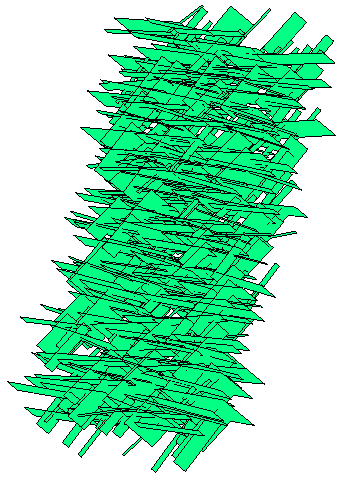
\includegraphics[width=0.4\textwidth]{../images/visu_maillage450Fracs.png}
%\caption{maillage450Fracs}
%\label{fig:maillage450Fracs}
%\end{figure}


\begin{figure}[p]
\centering
\subfloat[][Mesh.]
   {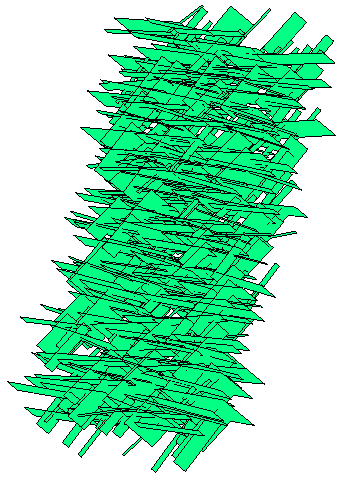
\includegraphics[width=.3\textwidth]{../images/visu_maillage450Fracs.png}} \quad
\subfloat[][Matrix compression for $\eta=1, \varepsilon=0.9$.]
   {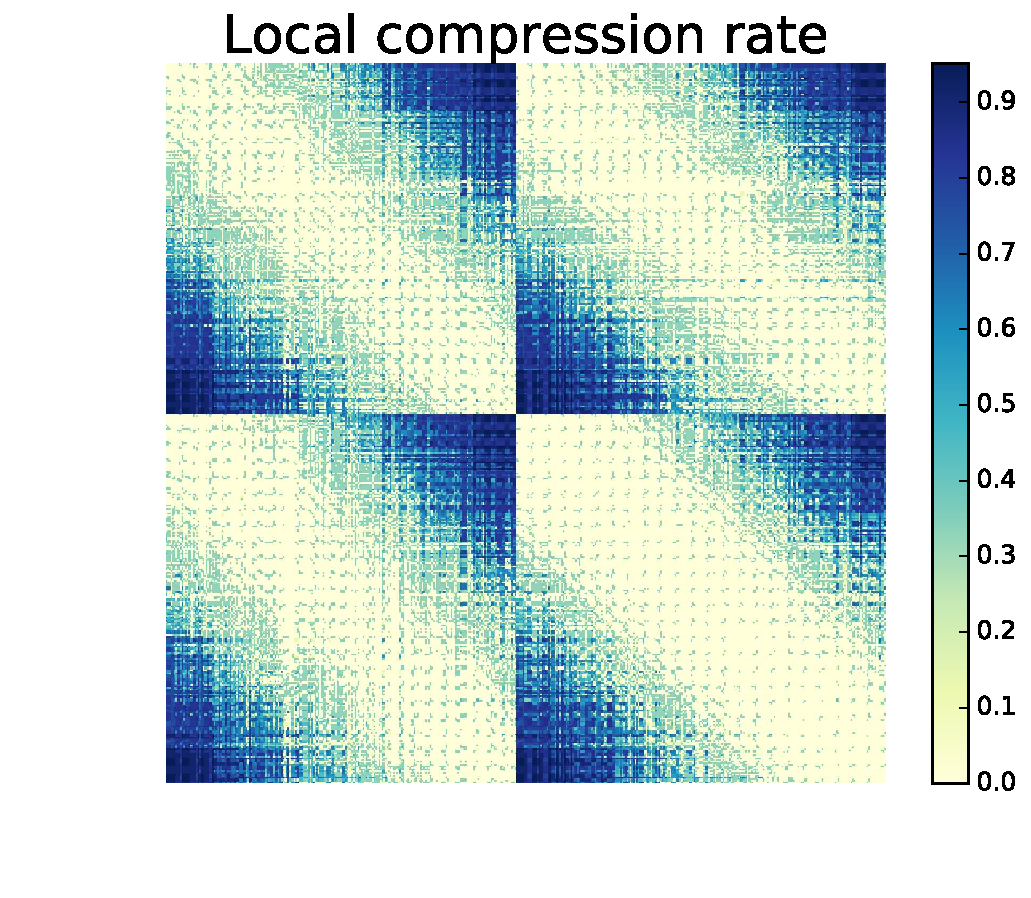
\includegraphics[width=.4\textwidth]{../images/graphe_mapp_output_local_comp_1_0,9_matrice450Fracs.pdf}\label{subfig:loccomp450Fracs}} \\
\subfloat[][Matrix compression for $\eta=10, \varepsilon=0.9$.]
   {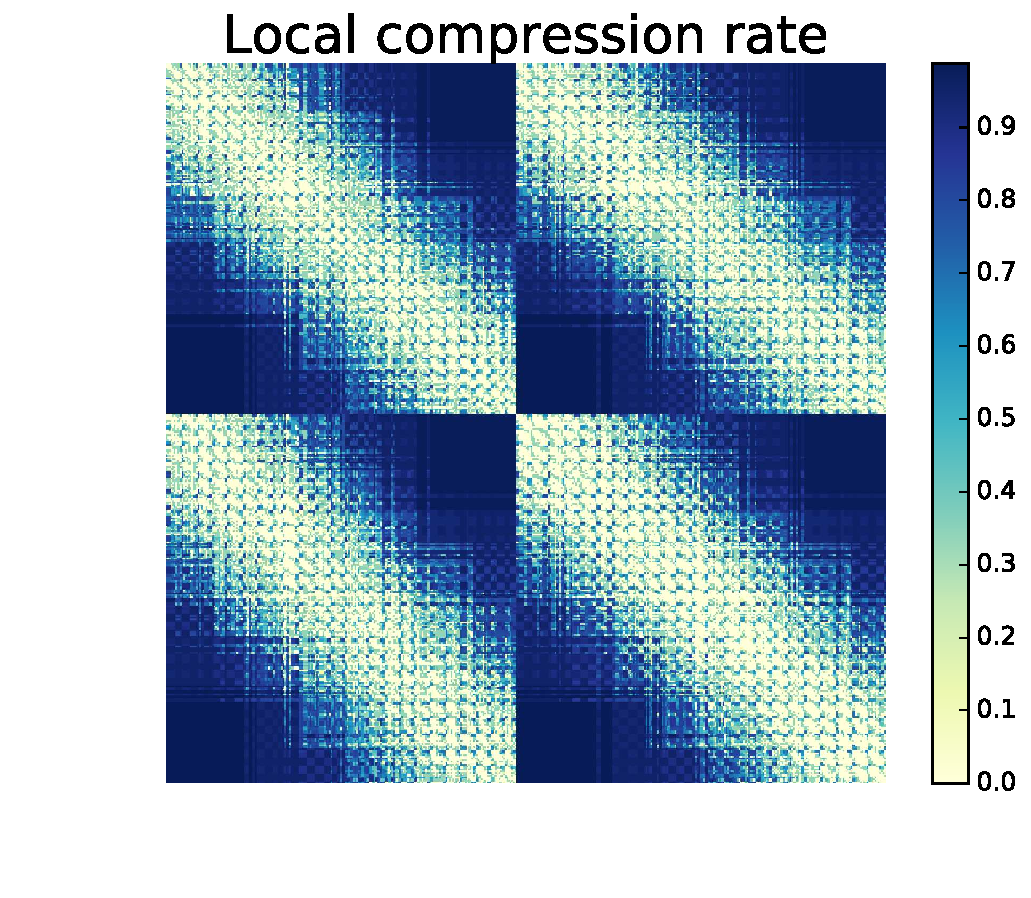
\includegraphics[width=.4\textwidth]{../images/graphe_mapp_output_local_comp_10_0,9_matrice450Fracs.pdf}}
\subfloat[][Matrix compression for $\eta=10, \varepsilon=1$.]
   {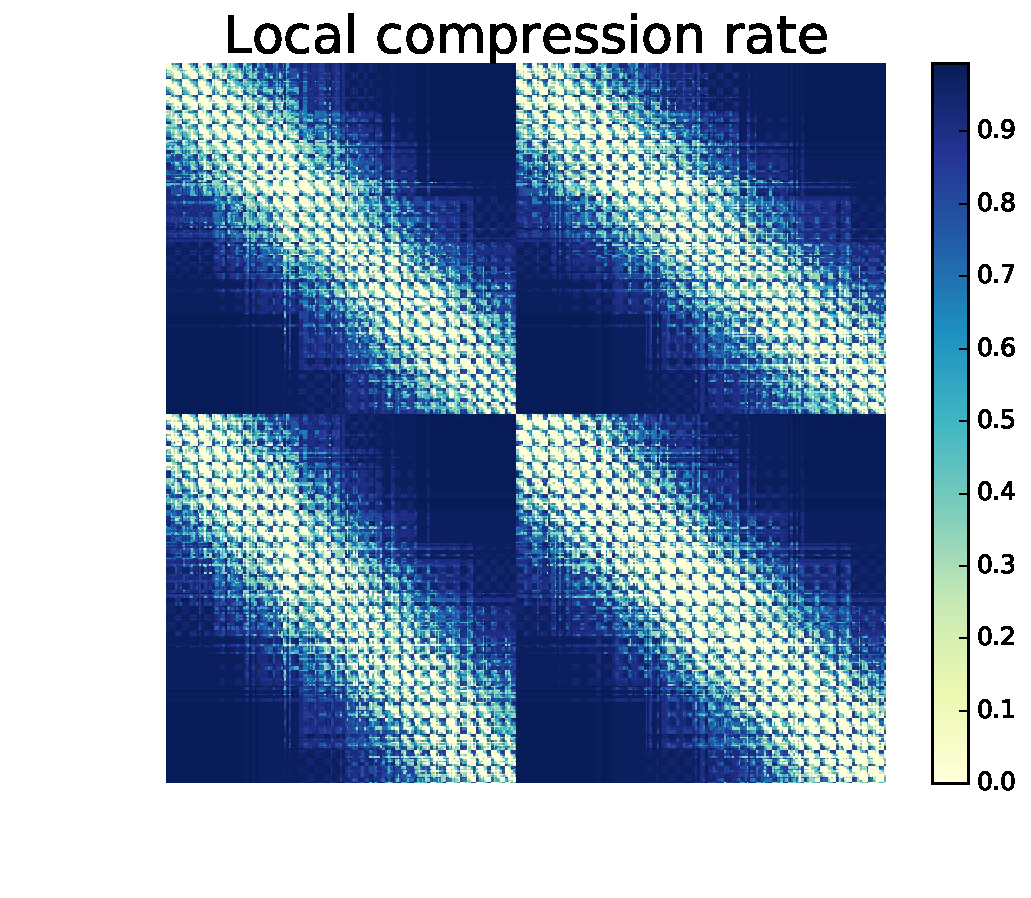
\includegraphics[width=.4\textwidth]{../images/graphe_mapp_output_local_comp_10_1_matrice450Fracs.pdf}} \\
\subfloat[][Errors and compression rates for different values of $\eta$ and $\varepsilon$.]
   {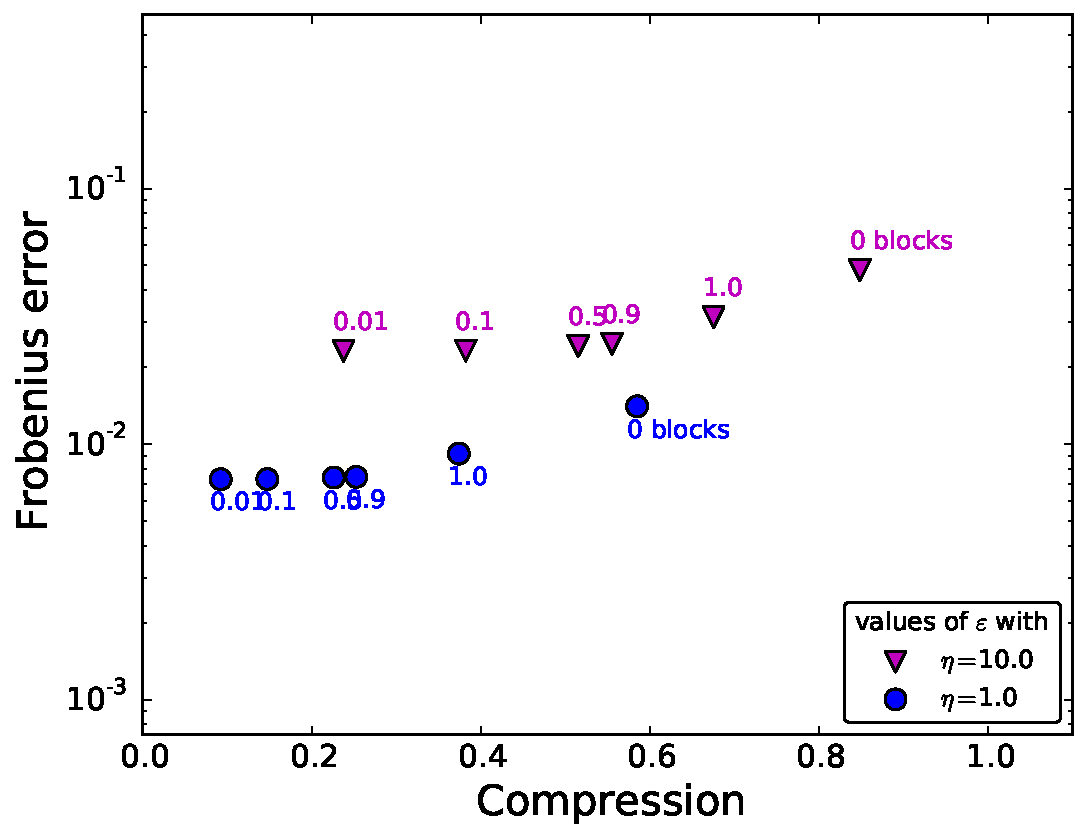
\includegraphics[width=.6\textwidth]{../images/graphe_compare_output_compression_18_08_2016matrice450Fracs.pdf}}
\caption{Results for the structure with $450$ fractures.}
\label{fig:450Fracs}
\end{figure}

\begin{figure}[p]
\centering
\subfloat[][Mesh.]
   {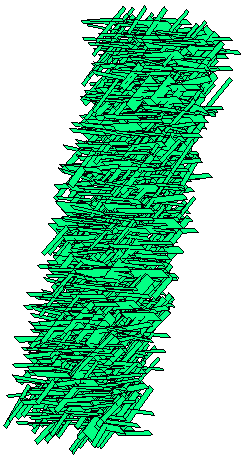
\includegraphics[width=.3\textwidth]{../images/visu_maillage1363Fracs.png}} \quad
\subfloat[][Matrix compression for $\eta=1, \varepsilon=0.9$.]
   {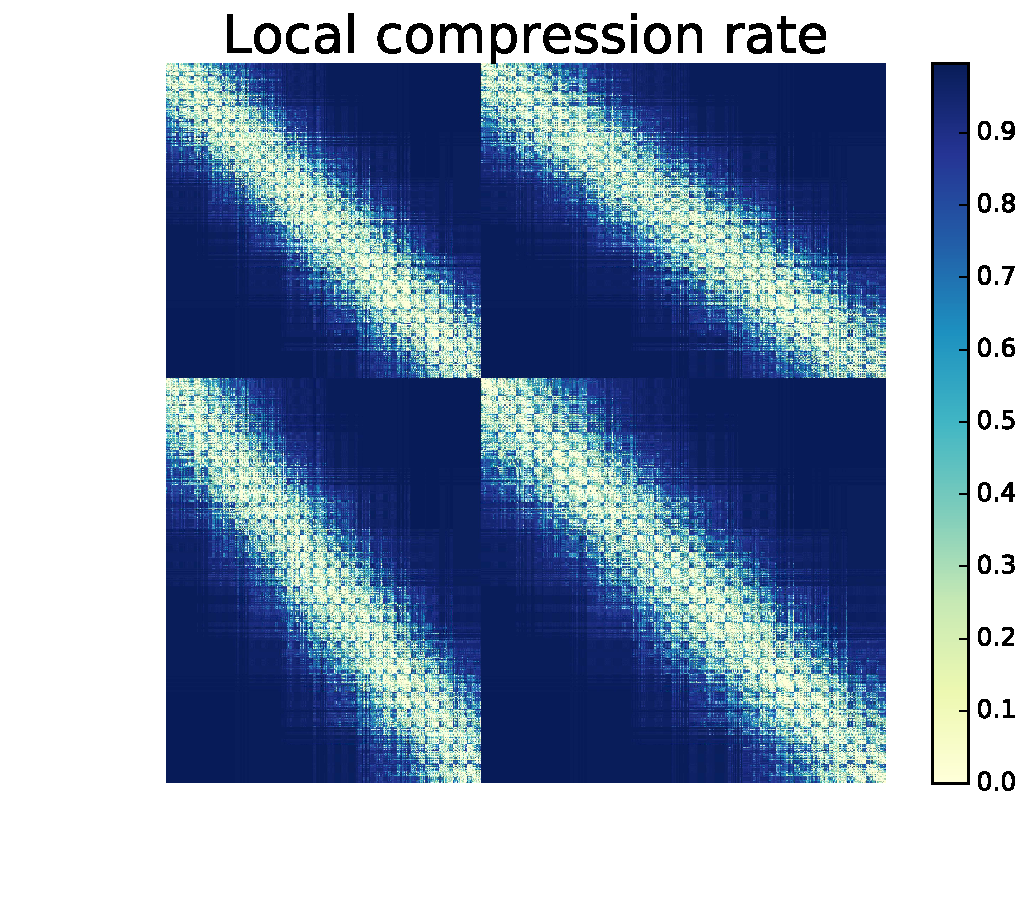
\includegraphics[width=.6\textwidth]{../images/graphe_mapp_output_local_comp_10_0,9_matrice1363Fracs.pdf}}\\
\subfloat[][Errors and compression rates for different values of $\eta$ and $\varepsilon$.]
   {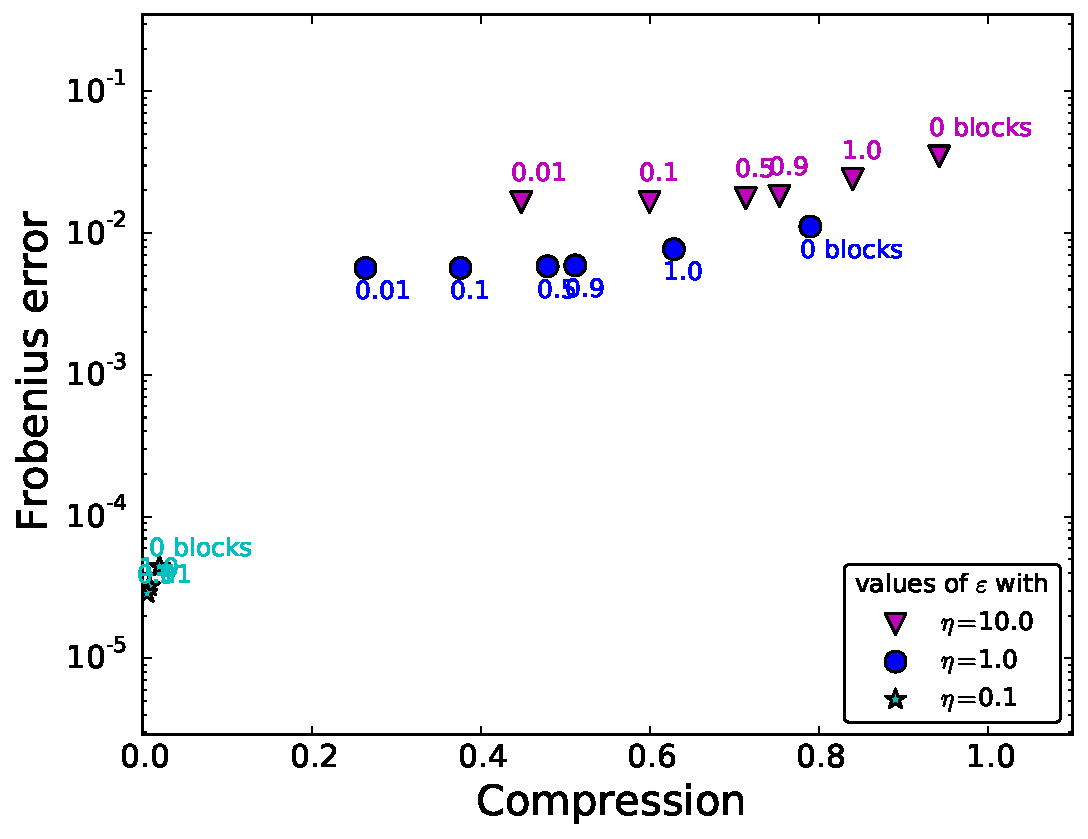
\includegraphics[width=.6\textwidth]{../images/graphe_compare_output_compression_18_08_2016matrice1363Fracs.pdf}}
\caption{Results for the structure with $1363$ fractures.}
\label{fig:1363Fracs}
\end{figure}

\begin{figure}[p]
\centering
\subfloat[][Mesh.]
   {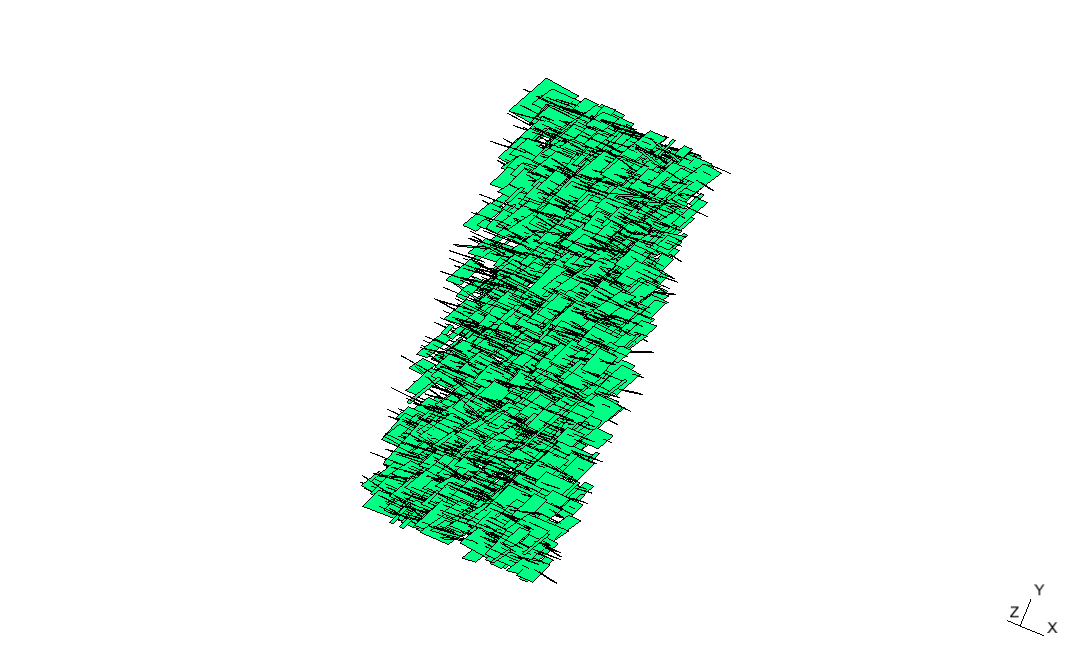
\includegraphics[width=.35\textwidth]{../images/visu_maillage1994Fracs.png}} 
\subfloat[][Errors and compression rates for different values of $\eta$ and $\varepsilon$.]
   {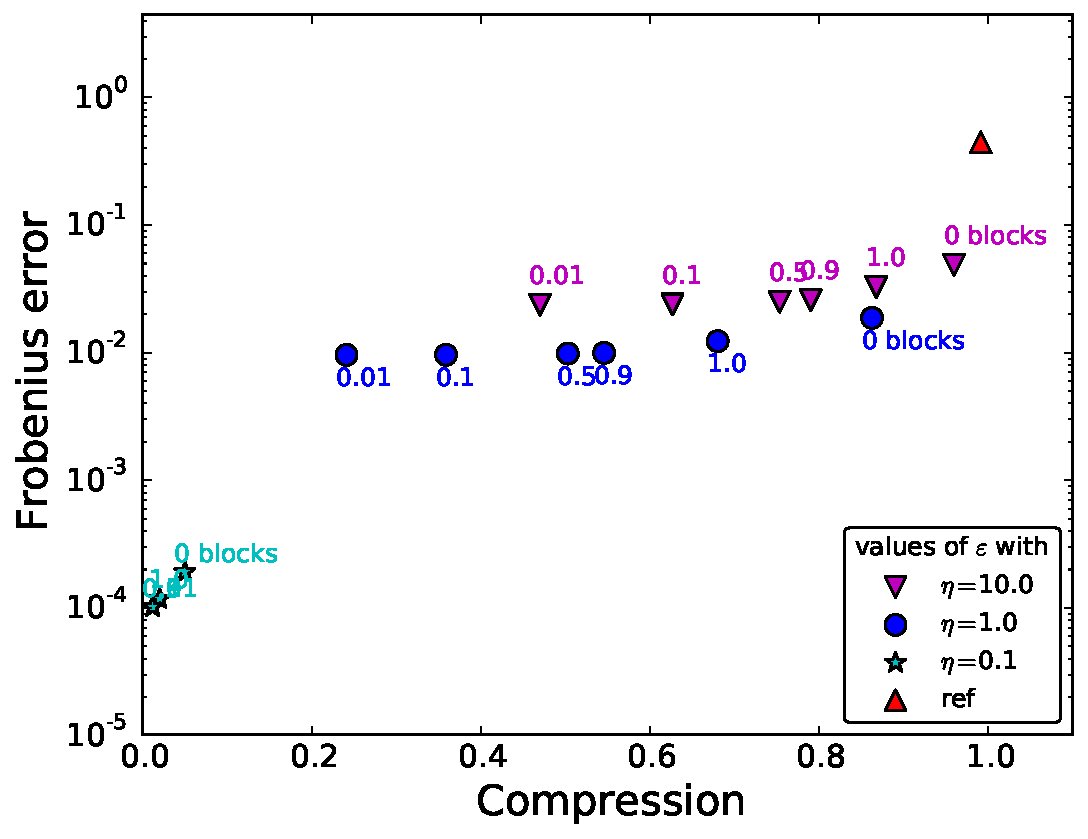
\includegraphics[width=.6\textwidth]{../images/graphe_compasparse_output_compression_18_08_2016matrice1994Fracs.pdf}}\\
\subfloat[][Times (s) to build the HM-ACA matrix and compression rates for different values of $\eta$ and $\varepsilon$.]
   {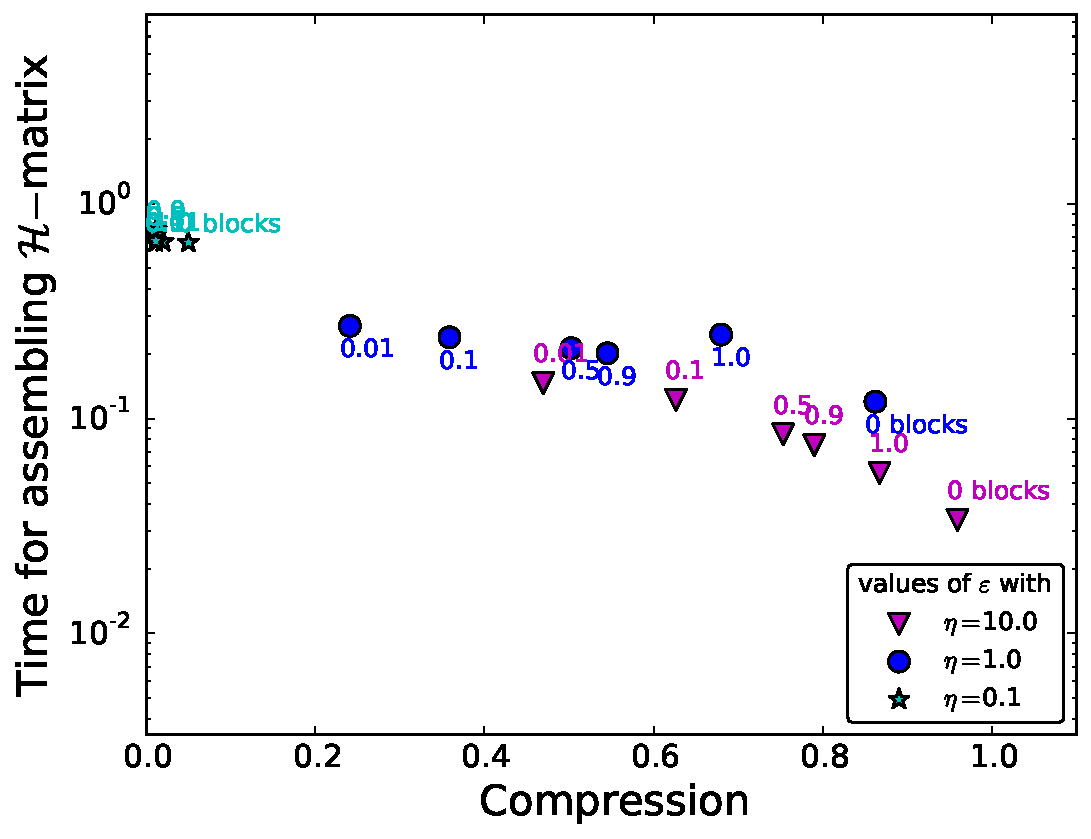
\includegraphics[width=.47\textwidth]{../images/graphe_tas_output_compression_18_08_2016matrice1994Fracs.pdf}} \;
\subfloat[][Times (s) for a matrix-vector product and compression rates for different values of $\eta$ and $\varepsilon$.]
   {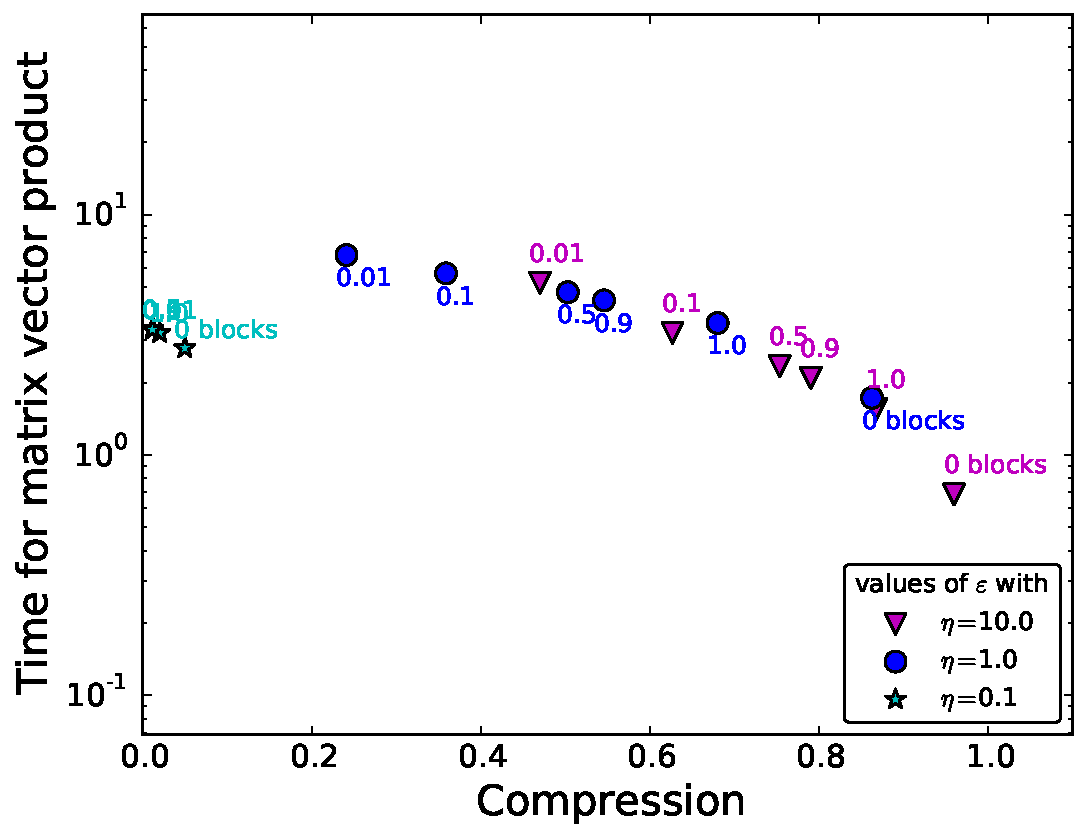
\includegraphics[width=.47\textwidth]{../images/graphe_tmv_output_compression_18_08_2016matrice1994Fracs.pdf}}
\caption{Results for the structure with $1994$ fractures.}
\label{fig:1994Fracs}
\end{figure}


%\begin{figure}[p]
%\centering
%\subfloat[][Mesh.]
%   {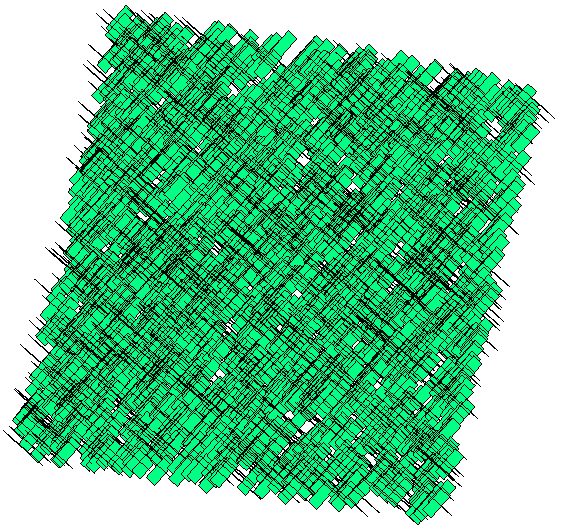
\includegraphics[width=.21\textwidth]{../images/visu_maillage2700FracsV1D1.png}} \qquad
%\subfloat[][Errors and compression rates.] %for different values of $\eta$ and $\varepsilon$.]
%   {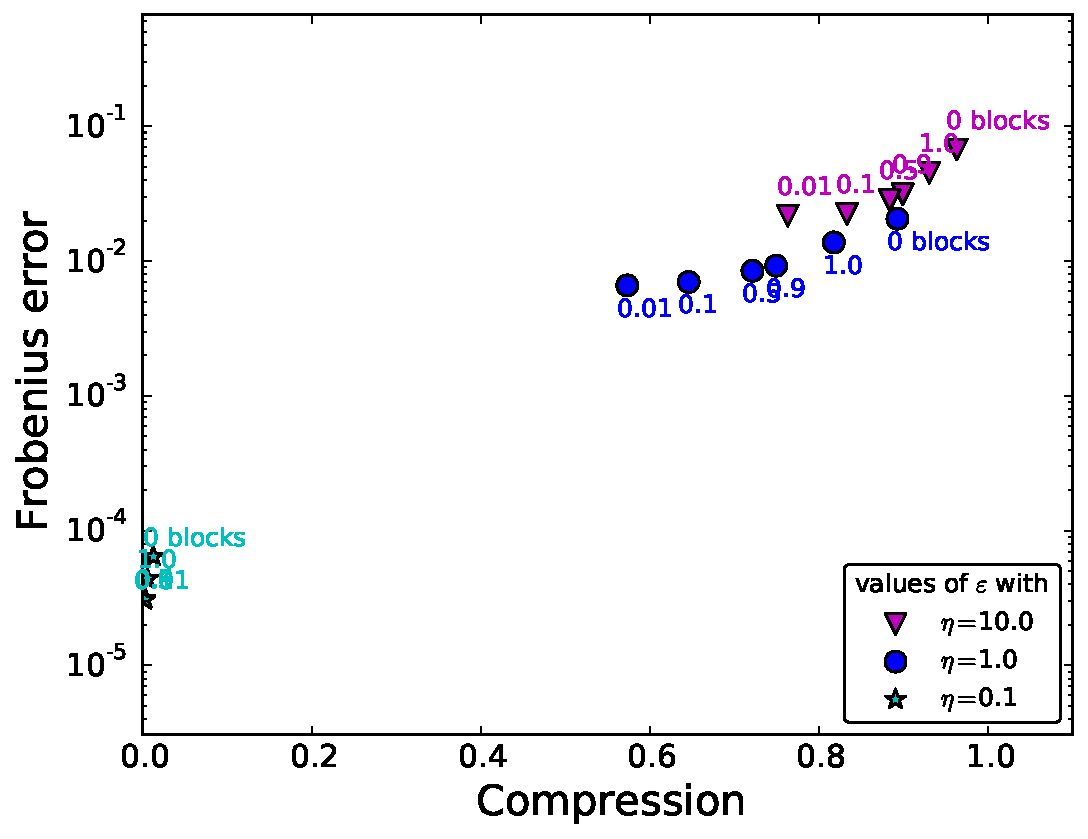
\includegraphics[width=.46\textwidth]{../images/graphe_compare_output_compression_18_08_2016matrice2700FracsV1D1.pdf}}
%\caption{Results for the structure with $2700$ fractures inside a volume $V_1=300\times300\times20$.}
%\label{fig:2700FracsV1D1}
%\end{figure}

\begin{figure}[p]
   \begin{minipage}[c]{.5\linewidth}
\centering
\subfloat[][Mesh.]
         {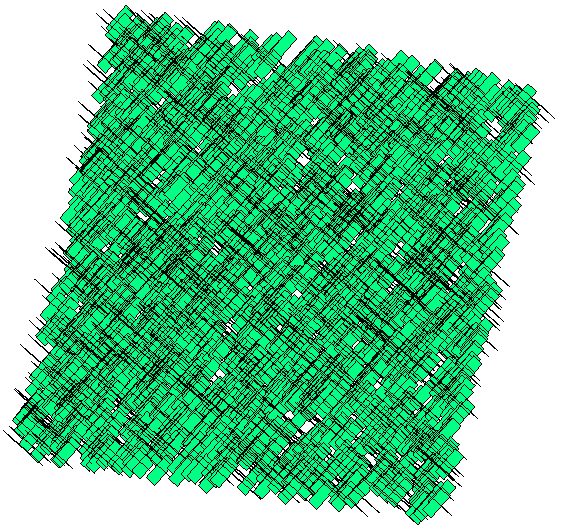
\includegraphics[width=.5\textwidth]{../images/visu_maillage2700FracsV1D1.png}}
   \end{minipage} \hfill
   \begin{minipage}[c]{.5\linewidth}
  \subfloat[][Errors and compression rates.] 
      {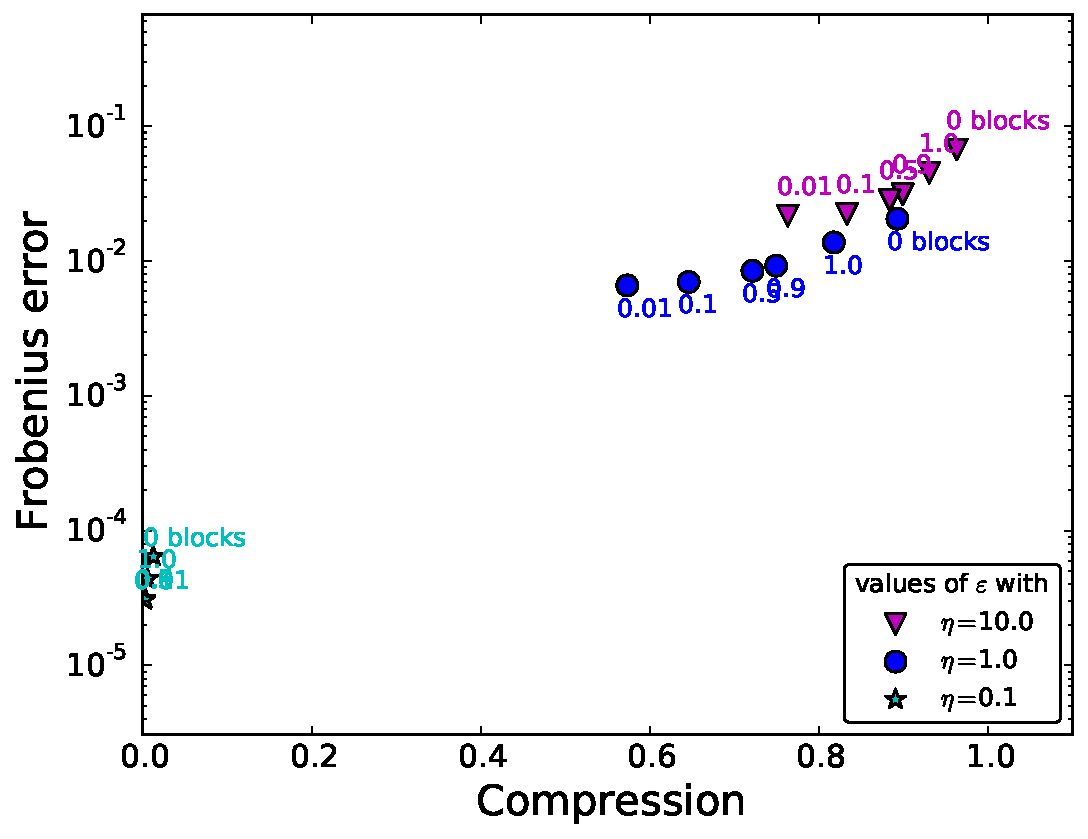
\includegraphics[width=.9\textwidth]{../images/graphe_compare_output_compression_18_08_2016matrice2700FracsV1D1.pdf}}
   \end{minipage}
   \caption{Results for the structure with $2700$ fractures inside a volume $V_1=300\times300\times20$.}
\label{fig:2700FracsV1D1}
\end{figure}

%\begin{figure}[p]
%\centering
%\subfloat[][Mesh.]
%   {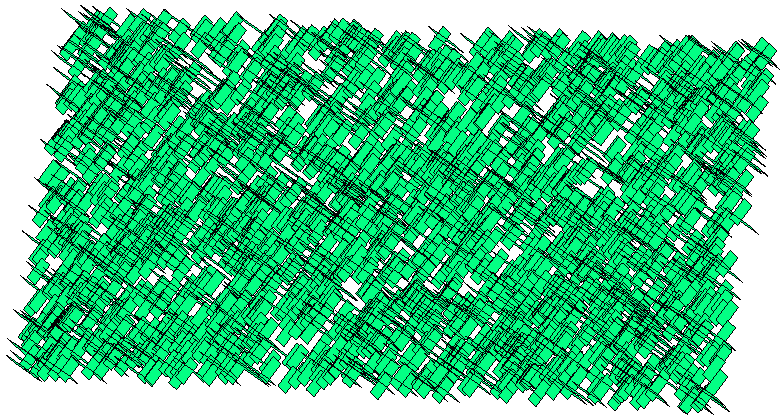
\includegraphics[width=.36\textwidth]{../images/visu_maillage2700FracsV2D2.png}} \qquad
%\subfloat[][Errors and compression rates.] %for different values of $\eta$ and $\varepsilon$.]
%   {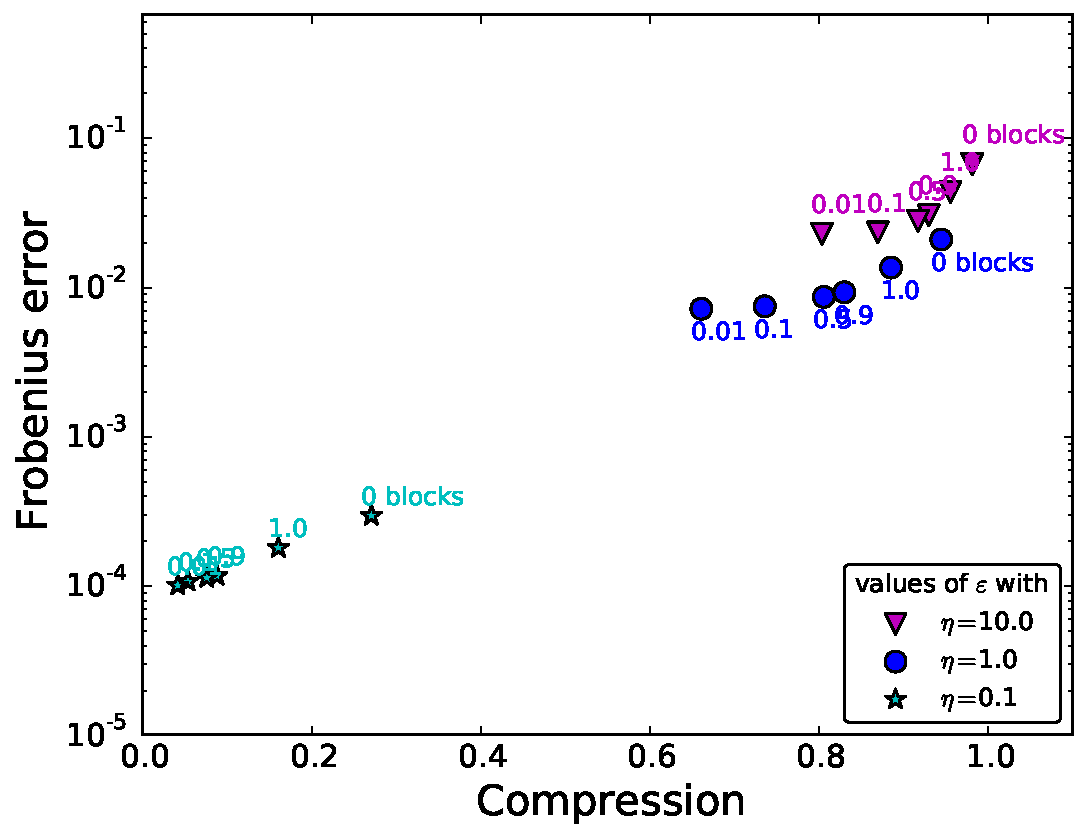
\includegraphics[width=.46\textwidth]{../images/graphe_compare_output_compression_18_08_2016matrice2700FracsV2D2.pdf}}
%\caption{Results for the structure with $2700$ fractures inside a volume $V_2=600\times300\times20$.}
%\label{fig:2700FracsV2D2}
%\end{figure}

\begin{figure}[p]
\begin{minipage}[c]{.5\linewidth}
\centering
\subfloat[][Mesh.]
         {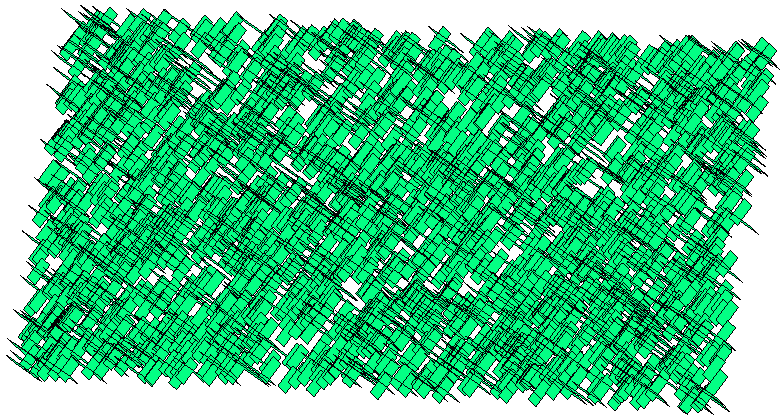
\includegraphics[width=.7\textwidth]{../images/visu_maillage2700FracsV2D2.png}}
   \end{minipage} \hfill
   \begin{minipage}[c]{.5\linewidth}
  \subfloat[][Errors and compression rates.] 
      {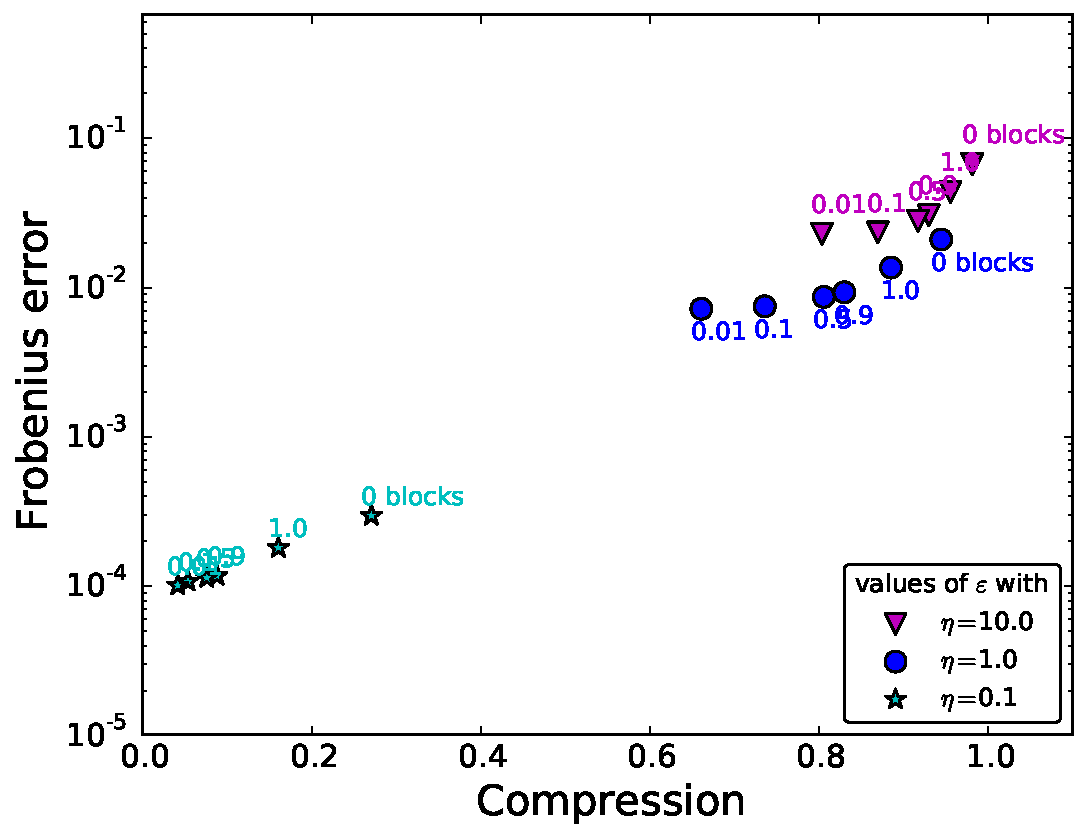
\includegraphics[width=.9\textwidth]{../images/graphe_compare_output_compression_18_08_2016matrice2700FracsV2D2.pdf}}
  \end{minipage}
   \caption{Results for the structure with $2700$ fractures inside a volume $V_2=600\times300\times20$.}
\label{fig:2700FracsV2D2}
\end{figure}

\begin{figure}[p]
 \begin{minipage}[c]{.5\linewidth}
\centering
\subfloat[][Mesh.]
   {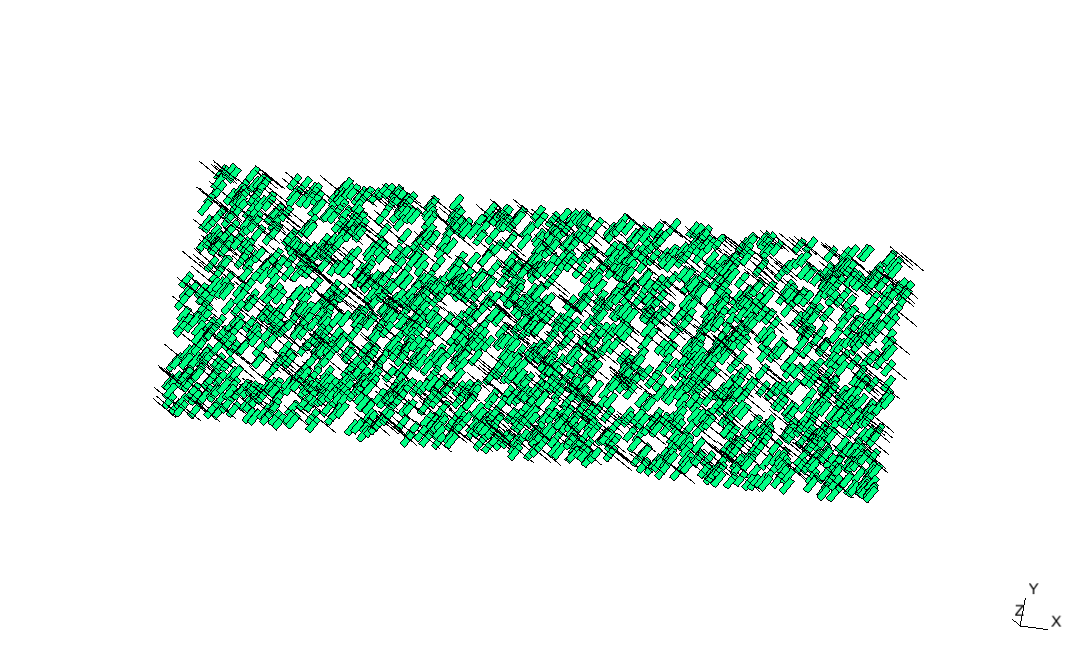
\includegraphics[width=.9\textwidth]{../images/visu_maillage2700FracsV3D3.png}}
\end{minipage} \hfill
\begin{minipage}[c]{.5\linewidth}
\subfloat[][Errors and compression rates.] %for different values of $\eta$ and $\varepsilon$.]
   {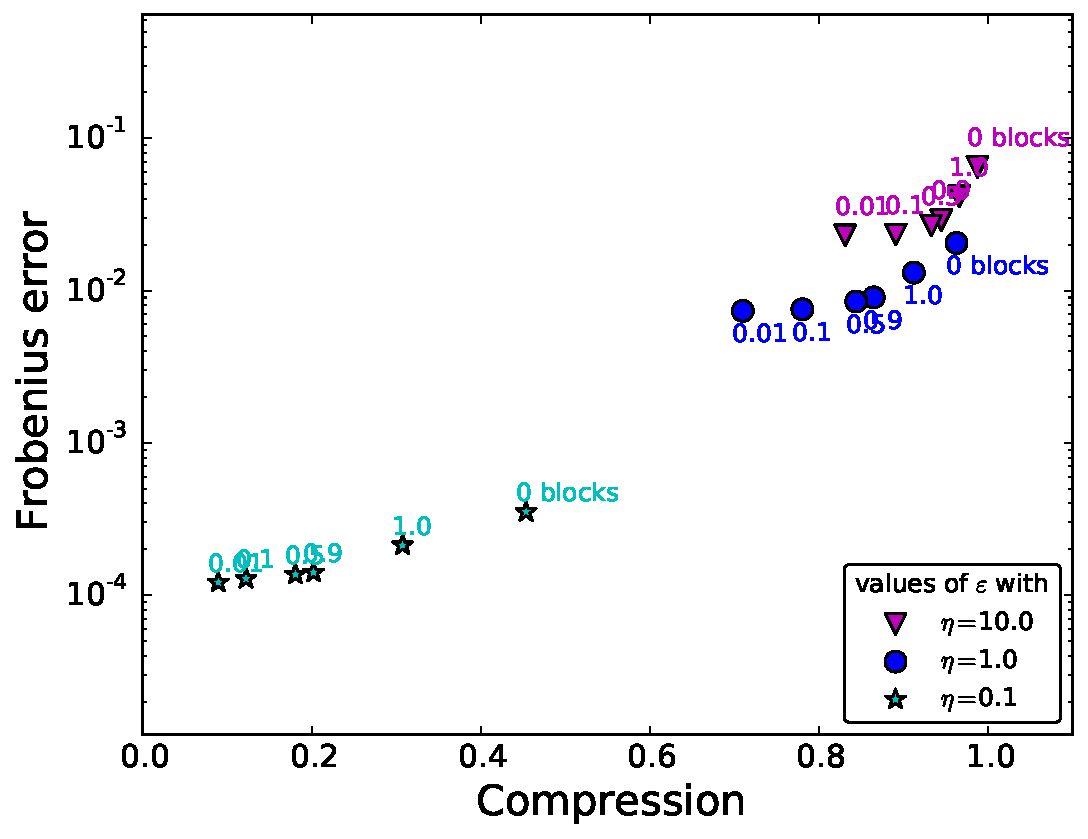
\includegraphics[width=.91\textwidth]{../images/graphe_compare_output_compression_18_08_2016matrice2700FracsV3D3.pdf}}
\end{minipage}
\caption{Results for the structure with $2700$ fractures inside a volume $V_3=900\times300\times20$.}
\label{fig:2700FracsV3D3}
\end{figure}


\begin{figure}[p]
\begin{minipage}[c]{.5\linewidth}
\centering
\subfloat[][Mesh.]
   {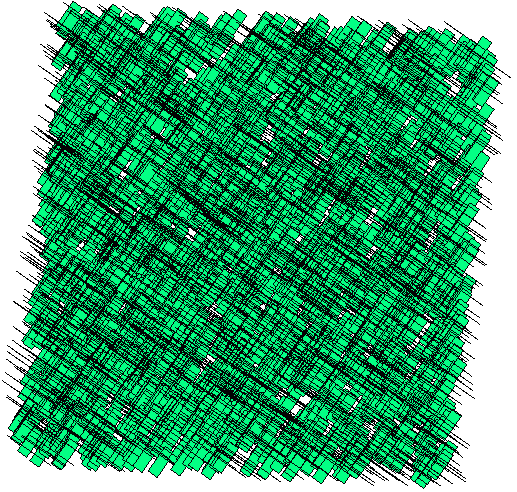
\includegraphics[width=.41\textwidth]{../images/visu_maillage3600FracsV1DN1.png}}
\end{minipage} \hfill
\begin{minipage}[c]{.5\linewidth}
\subfloat[][Errors and compression rates.] %for different values of $\eta$ and $\varepsilon$.]
   {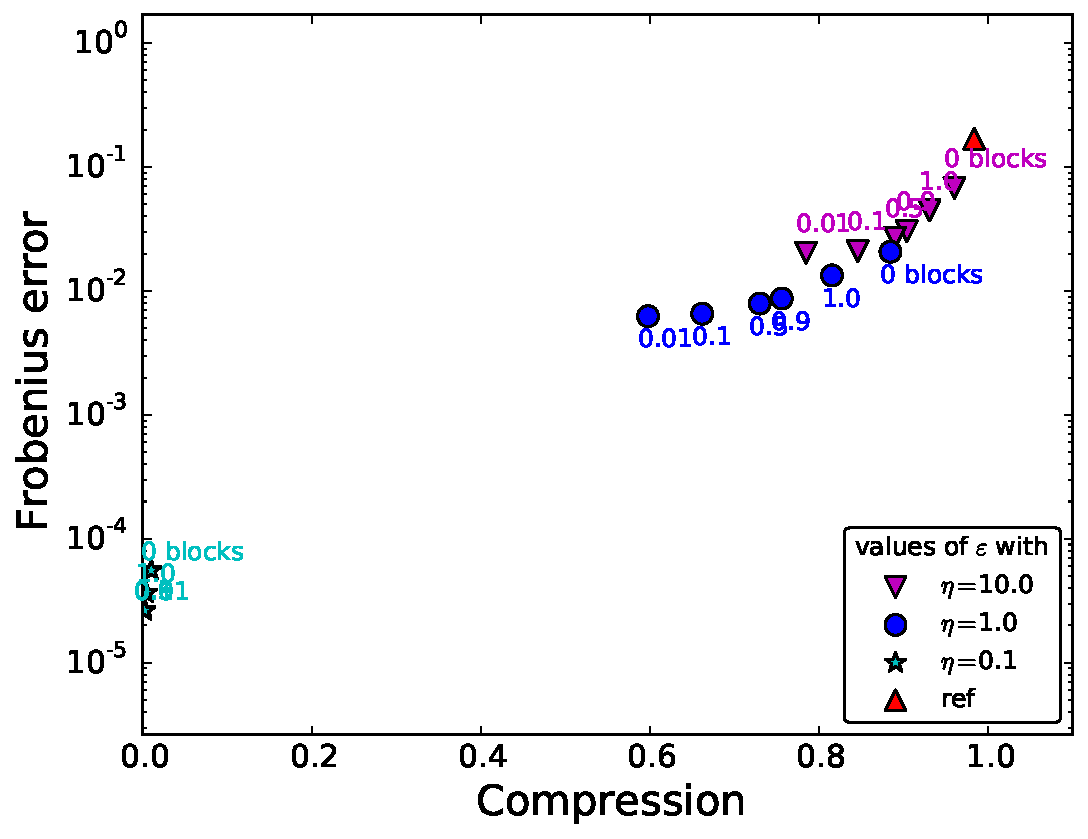
\includegraphics[width=.9\textwidth]{../images/graphe_compasparse_output_compression_18_08_2016matrice3600FracsV1DN1.pdf}}
\end{minipage}
\caption{Results for the structure with $3600$ fractures inside a volume $V_1=300\times300\times20$.}
\label{fig:3600FracsV1DN1}
\end{figure}

\begin{figure}[p]
\begin{minipage}[c]{.5\linewidth}
\centering
\subfloat[][Mesh.]
   {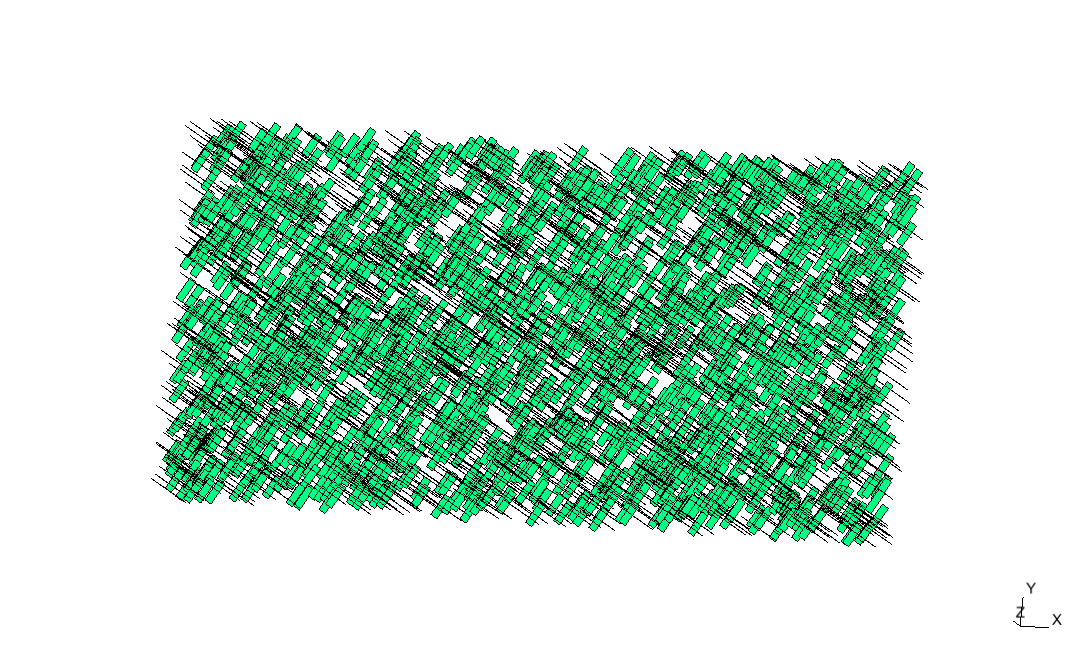
\includegraphics[width=.7\textwidth]{../images/visu_maillage3600FracsV2DN2.png}} 
\end{minipage} \hfill
\begin{minipage}[c]{.5\linewidth}
\subfloat[][Errors and compression rates.] %for different values of $\eta$ and $\varepsilon$.]
   {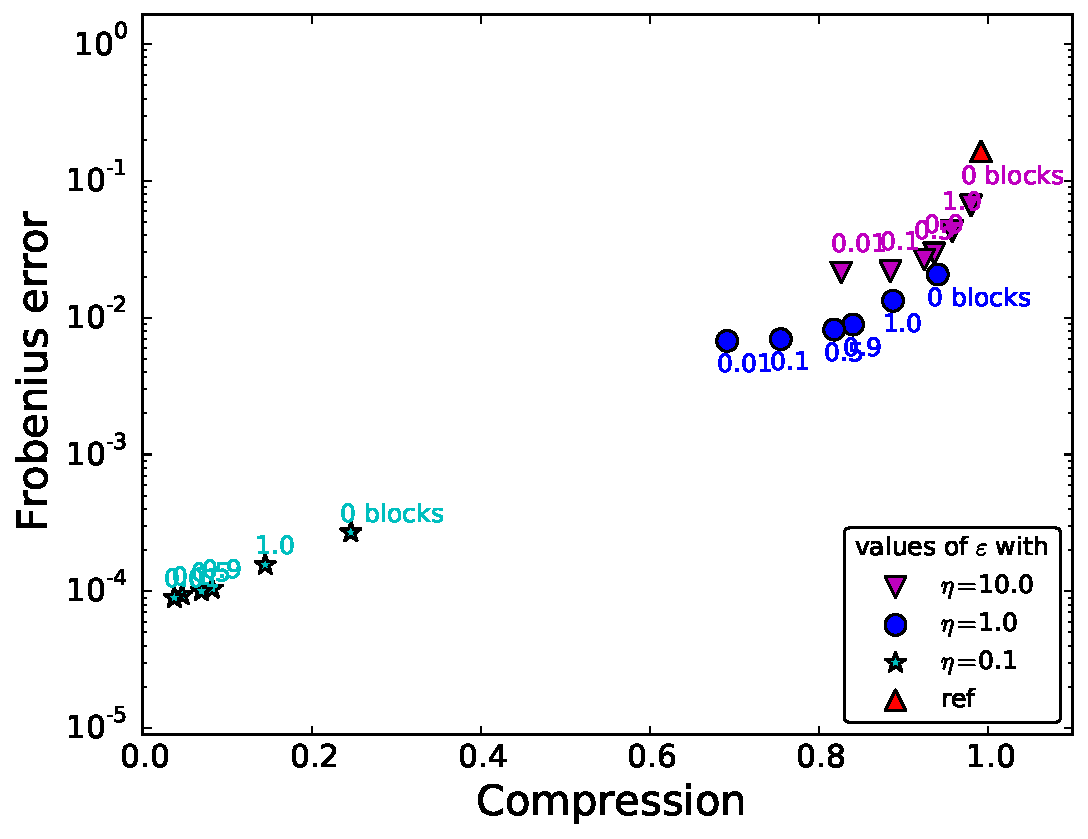
\includegraphics[width=.9\textwidth]{../images/graphe_compasparse_output_compression_18_08_2016matrice3600FracsV2DN2.pdf}}
\end{minipage}
\caption{Results for the structure with $3600$ fractures inside a volume $V_2=600\times300\times20$.}
\label{fig:3600FracsV2DN2}
\end{figure}

\begin{figure}[p]
\begin{minipage}[c]{.5\linewidth}
\centering
\subfloat[][Mesh.]
   {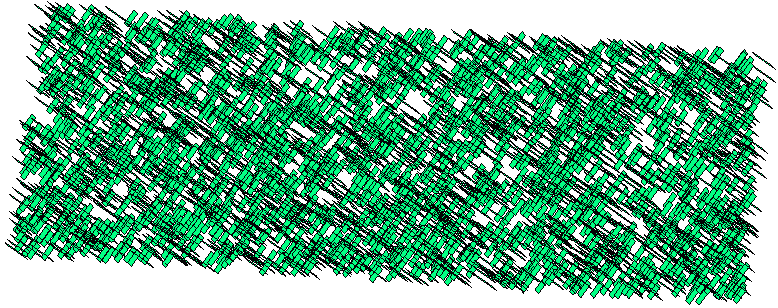
\includegraphics[width=.9\textwidth]{../images/visu_maillage3600FracsV3DN3.png}}
\end{minipage} \hfill
\begin{minipage}[c]{.5\linewidth}
\subfloat[][Errors and compression rates.] %for different values of $\eta$ and $\varepsilon$.]
   {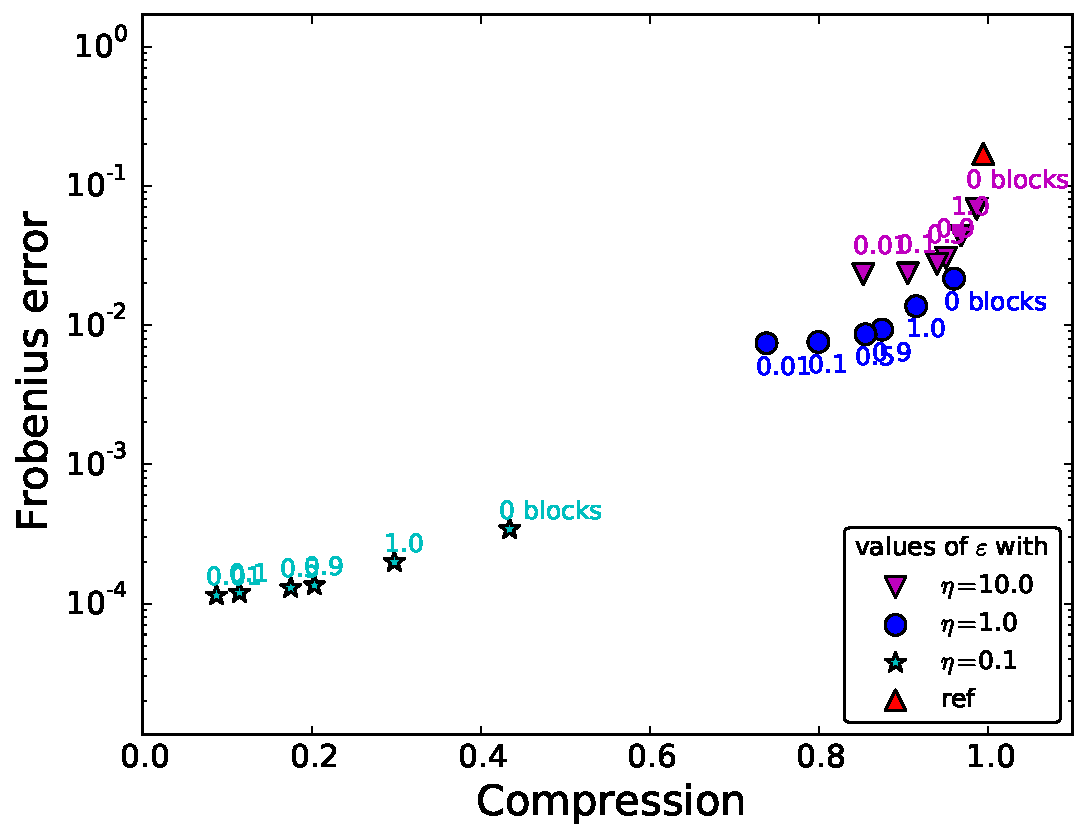
\includegraphics[width=.9\textwidth]{../images/graphe_compasparse_output_compression_18_08_2016matrice3600FracsV3DN3.pdf}}
\end{minipage}
\caption{Results for the structure with $3600$ fractures inside a volume $V_3=900\times300\times20$.}
\label{fig:3600FracsV3DN3}
\end{figure}


\begin{figure}[p]
\centering
\subfloat[][Mesh.]
   {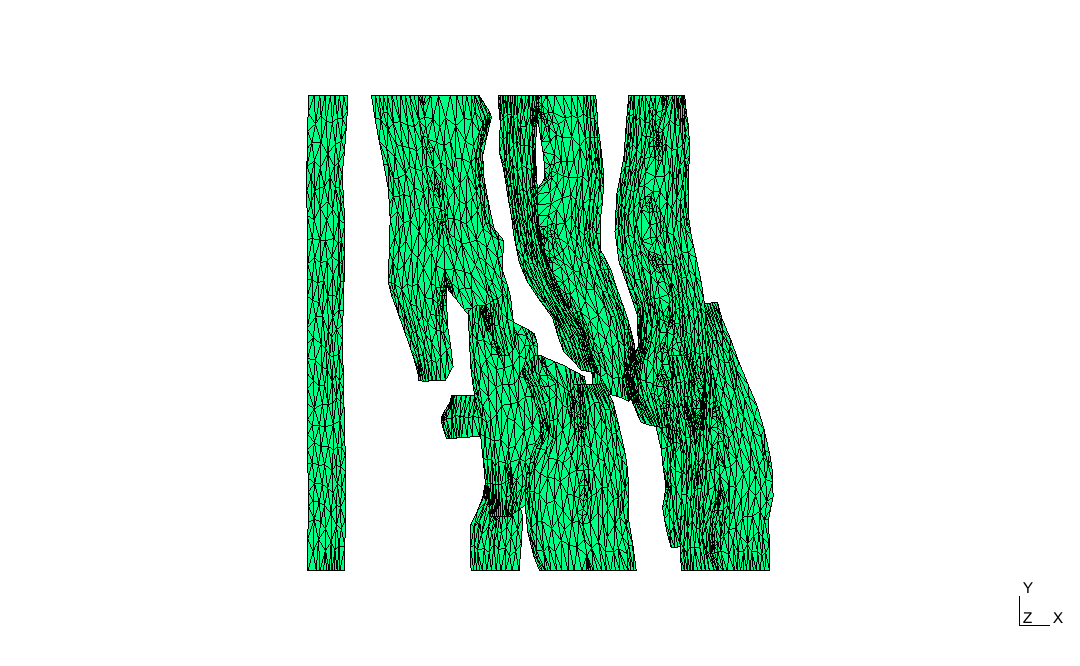
\includegraphics[width=.41\textwidth]{../images/visu_maillage5364FracsTriangles.png}}
\subfloat[][Errors and compression rates for different values of $\eta$ and $\varepsilon$.]
   {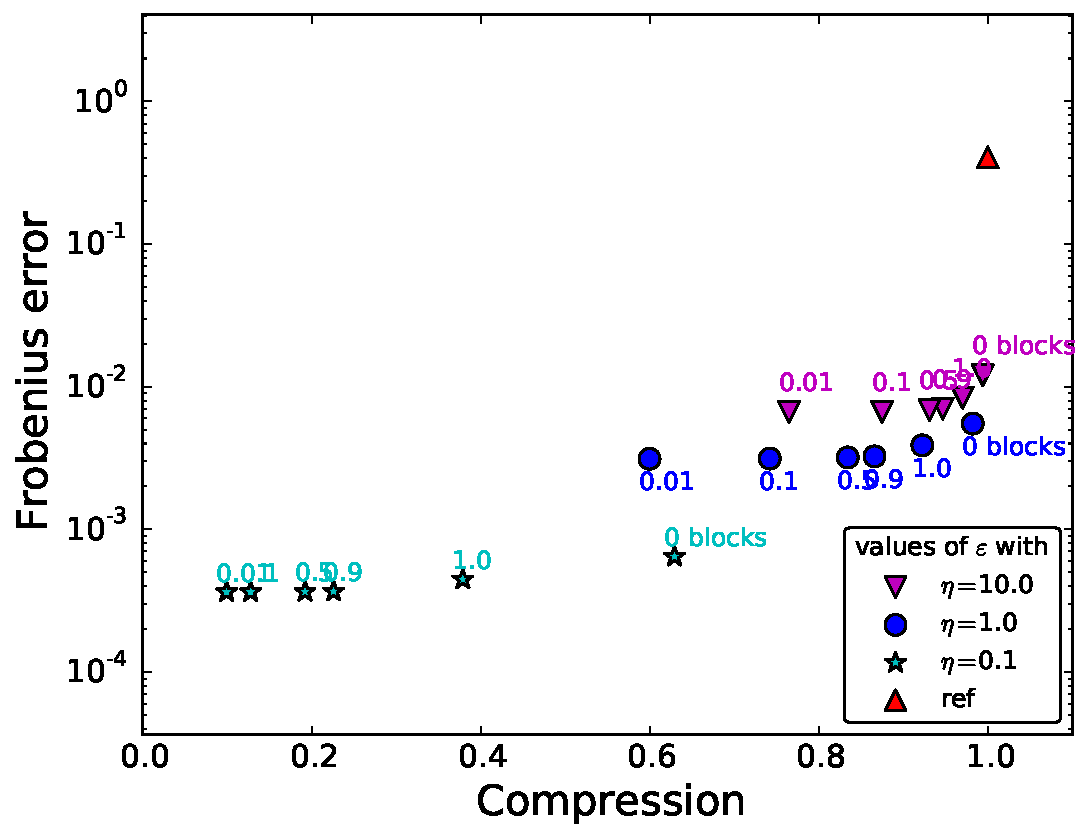
\includegraphics[width=.58\textwidth]{../images/graphe_compasparse_output_compression_18_08_2016matrice5364FracsTriangles.pdf}}\\
\subfloat[][Times (s) to build the HM-ACA matrix and compression rates for different values of $\eta$ and $\varepsilon$.]
   {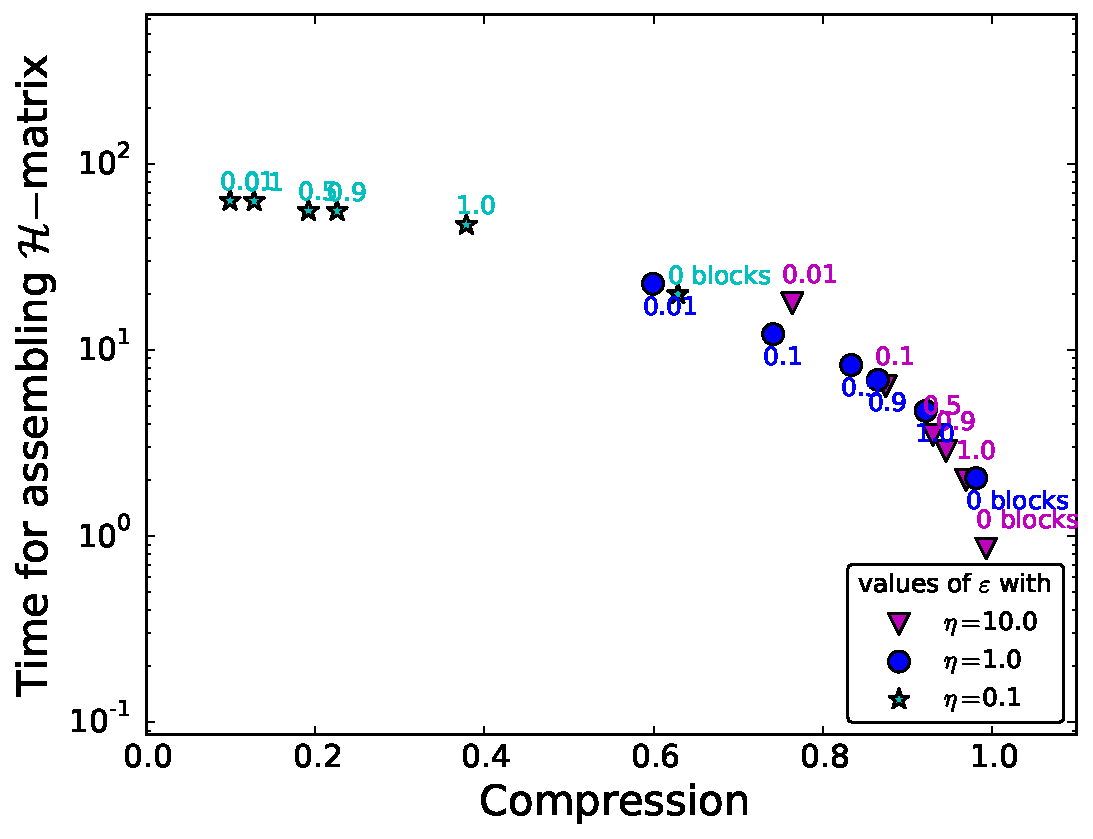
\includegraphics[width=.47\textwidth]{../images/graphe_tas_output_compression_18_08_2016matrice5364FracsTriangles.pdf}} \;
\subfloat[][Times (s) for a matrix-vector product and compression rates for different values of $\eta$ and $\varepsilon$.]
   {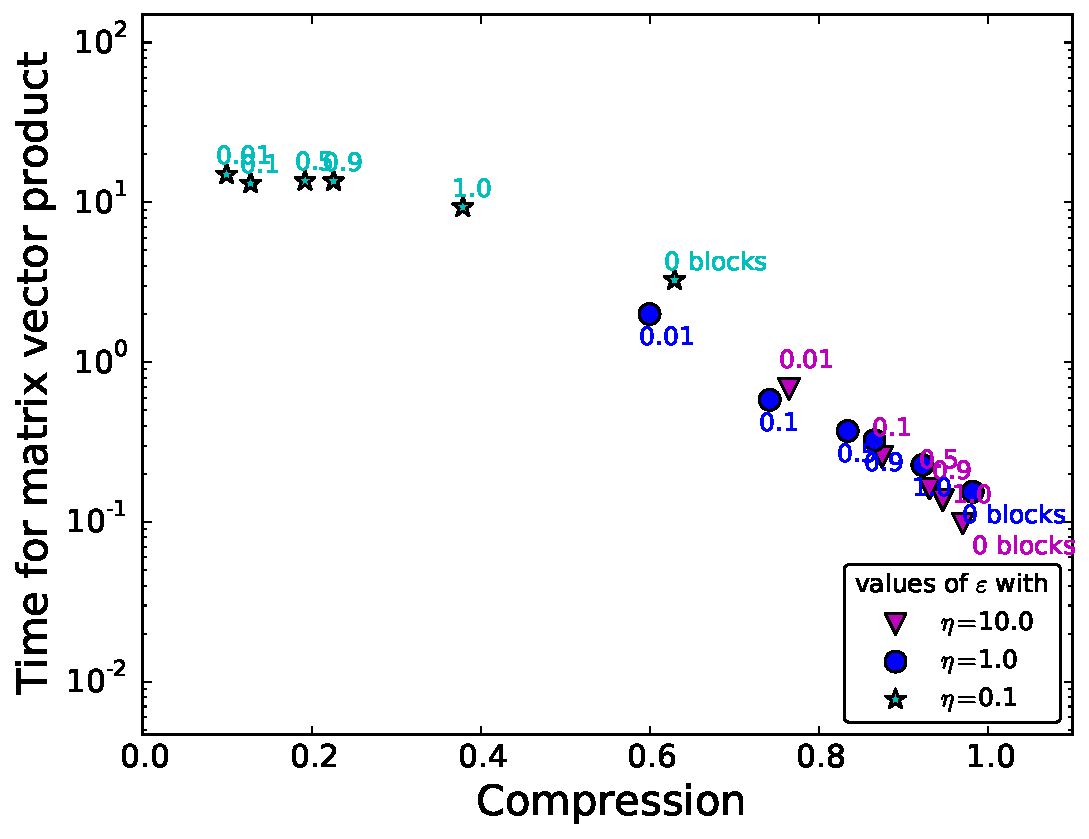
\includegraphics[width=.47\textwidth]{../images/graphe_tmv_output_compression_18_08_2016matrice5364FracsTriangles.pdf}}
\caption{Results for the structure of faults with $5364$ mesh triangles.}
\label{fig:5364FracsTriangles}
\end{figure}



